\documentclass[usletter, 12pt]{article}
\usepackage{amsmath}
\usepackage{enumitem}
\usepackage{graphicx}
\usepackage{pdfpages}
\graphicspath{ {images/} }


\begin{document}


\begin{enumerate}[leftmargin=0em, label=\textbf{\arabic*}.]
  \setcounter{enumi}{3} % remove this if you want to add other solutions 
  \item \textbf{Solution}:\\
    \begin{enumerate}[leftmargin=2em, label=(\textbf{\alph*})]
    \item
    \item For these parts we use mathematica to display the first five Legendre
      polynomials and then use the Rodrigues' formula (shown in class) to verify
      that the formula works. 
      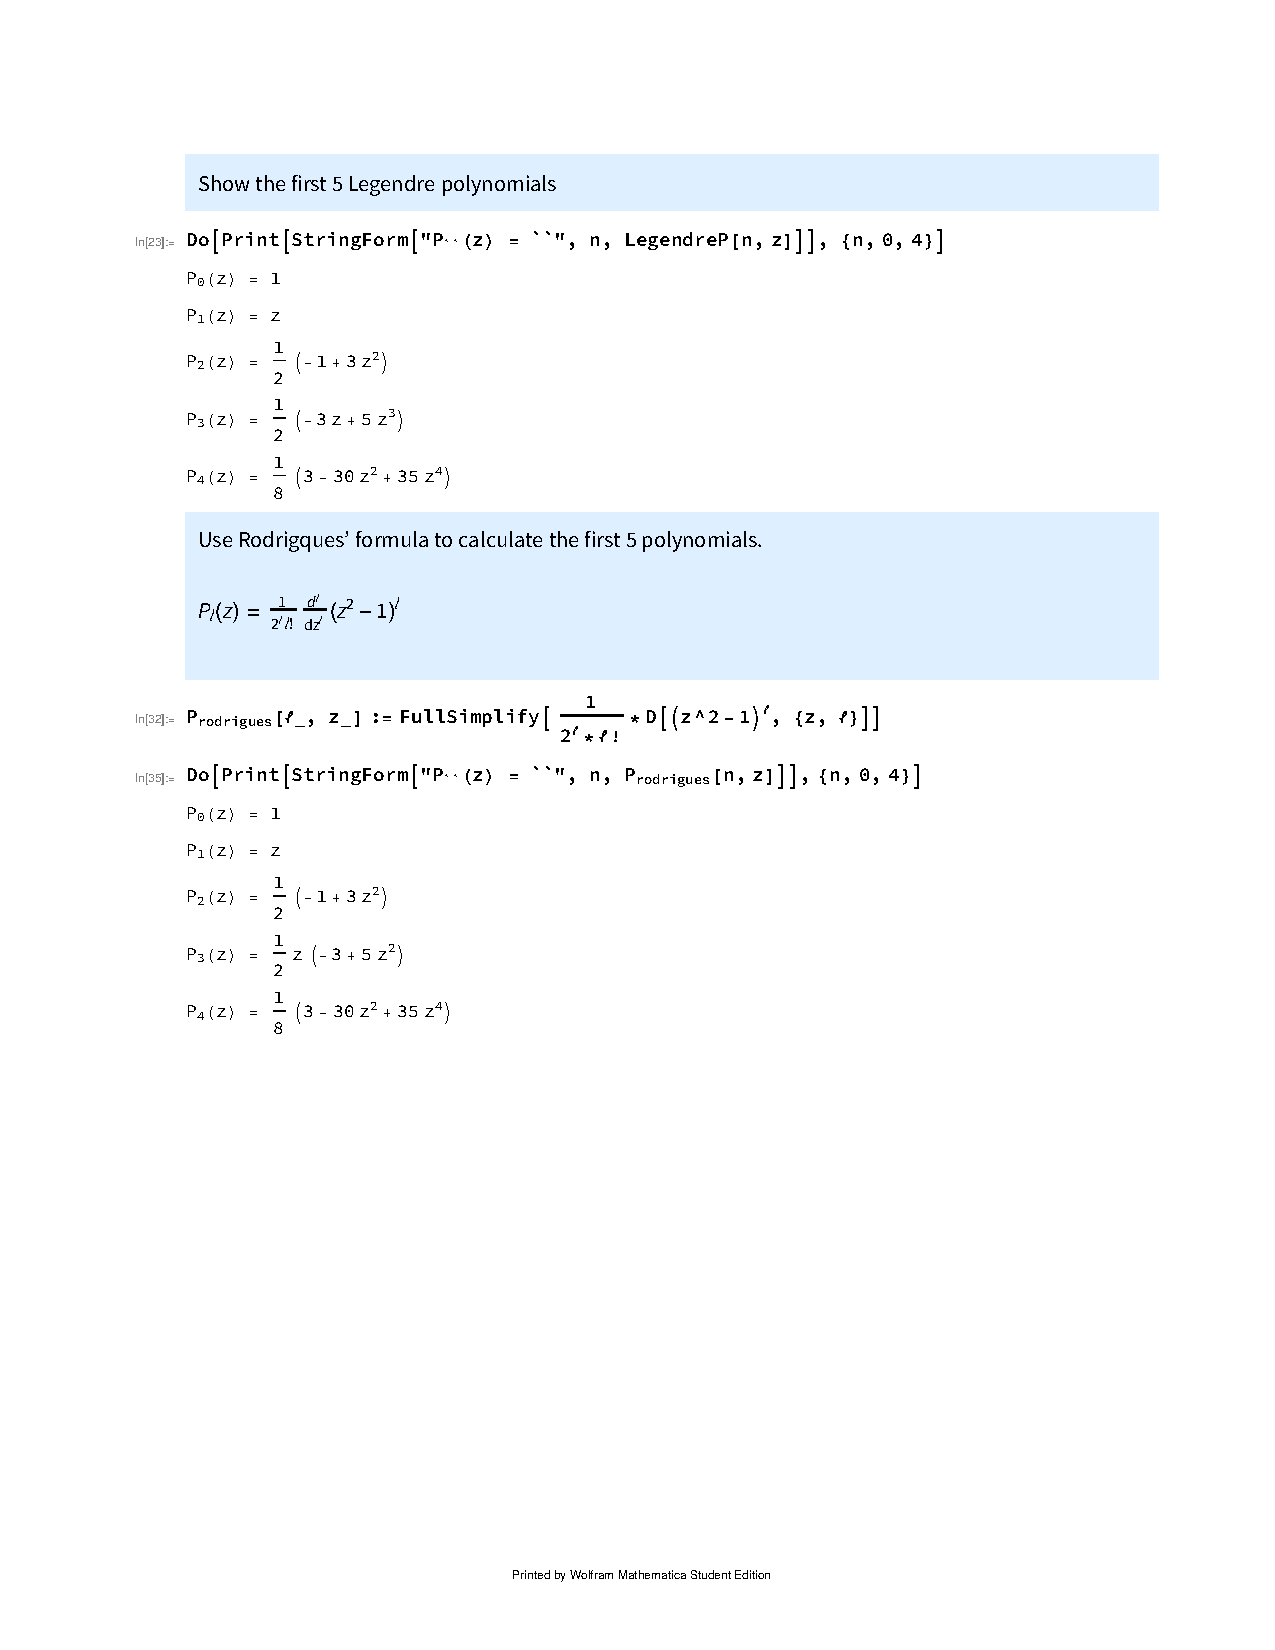
\includepdf[pages=-]{a_and_b.pdf}

    \item The recurrence relations for Legendre Polynomials (and other
      special functions) are \textbf{NOT} the recurrence relations for
      Legendre's equation. \textit{Be careful}.\\

      There are two important recurrence relations for the Legendre polynomials.
      They are
      \begin{align}
        (\ell+1)P_{\ell+1} &= (2\ell+1)zP_\ell-\ell P_{\ell-1} \\
        \frac{z^2-1}{\ell}P_\ell' &= zP_\ell - P_{\ell-1}
      \end{align}
      We are given that $P_0(z)=1$ and $P_1(z)=z$. Using, the first recurrence
      relations, we find that
      \begin{align}
        P_2 &= \frac{3zP_1-P_0}{2} = \frac{1}{2}(3z^2-z) \\
        P_3 &= \frac{5zP_2-2P_1}{3} = \frac{5z\left( \frac{1}{2}(3z^2-z) \right)-2z}{3} = \frac{1}{2}\left( 5z^3-3z \right)
      \end{align}

      Now we can use the second recurrence relation to find $P_3'(z)$.
      \begin{align}
        P_3'(z) &= \frac{3}{z^2-1}\left( zP_3-P_2 \right) \\
                &=\frac{3}{z^2-1}\left(z \frac{1}{2}\left( 5z^3-3z \right) -  \frac{1}{2}(3z^2-z) \right) \\
                &= \frac{3}{2(z^2-1)}-\frac{9z^2}{(z^2-1)}+\frac{15z^4}{2(z^2-1)}\\
                &= \frac{3}{2}\frac{(z^2-1)(5z^2-1)}{(z^2-1)} \\ 
                &= \frac{3}{2}\left( 5z^2-1 \right)
      \end{align}

      Thus we have found expressions for $P_3(z)$ and $P_3'(z)$ using the two
      recurrence relations. You are encouraged to double check your solution for
      $P_3'(z)$ by differentiating your result for $P_3(z)$
    \end{enumerate}
    
\end{enumerate}
\end{document}
